\documentclass{article}
\usepackage[utf8]{inputenc}
\usepackage{graphicx}
\graphicspath{ {./images/} }
\usepackage{listings}

\title{CS 590 Assignment 3}
\author{Luke Jiang (jiang700@purdue.edu) }
\date{March 7, 2021}

\begin{document}

\maketitle

\section{Screenshot of container instance}
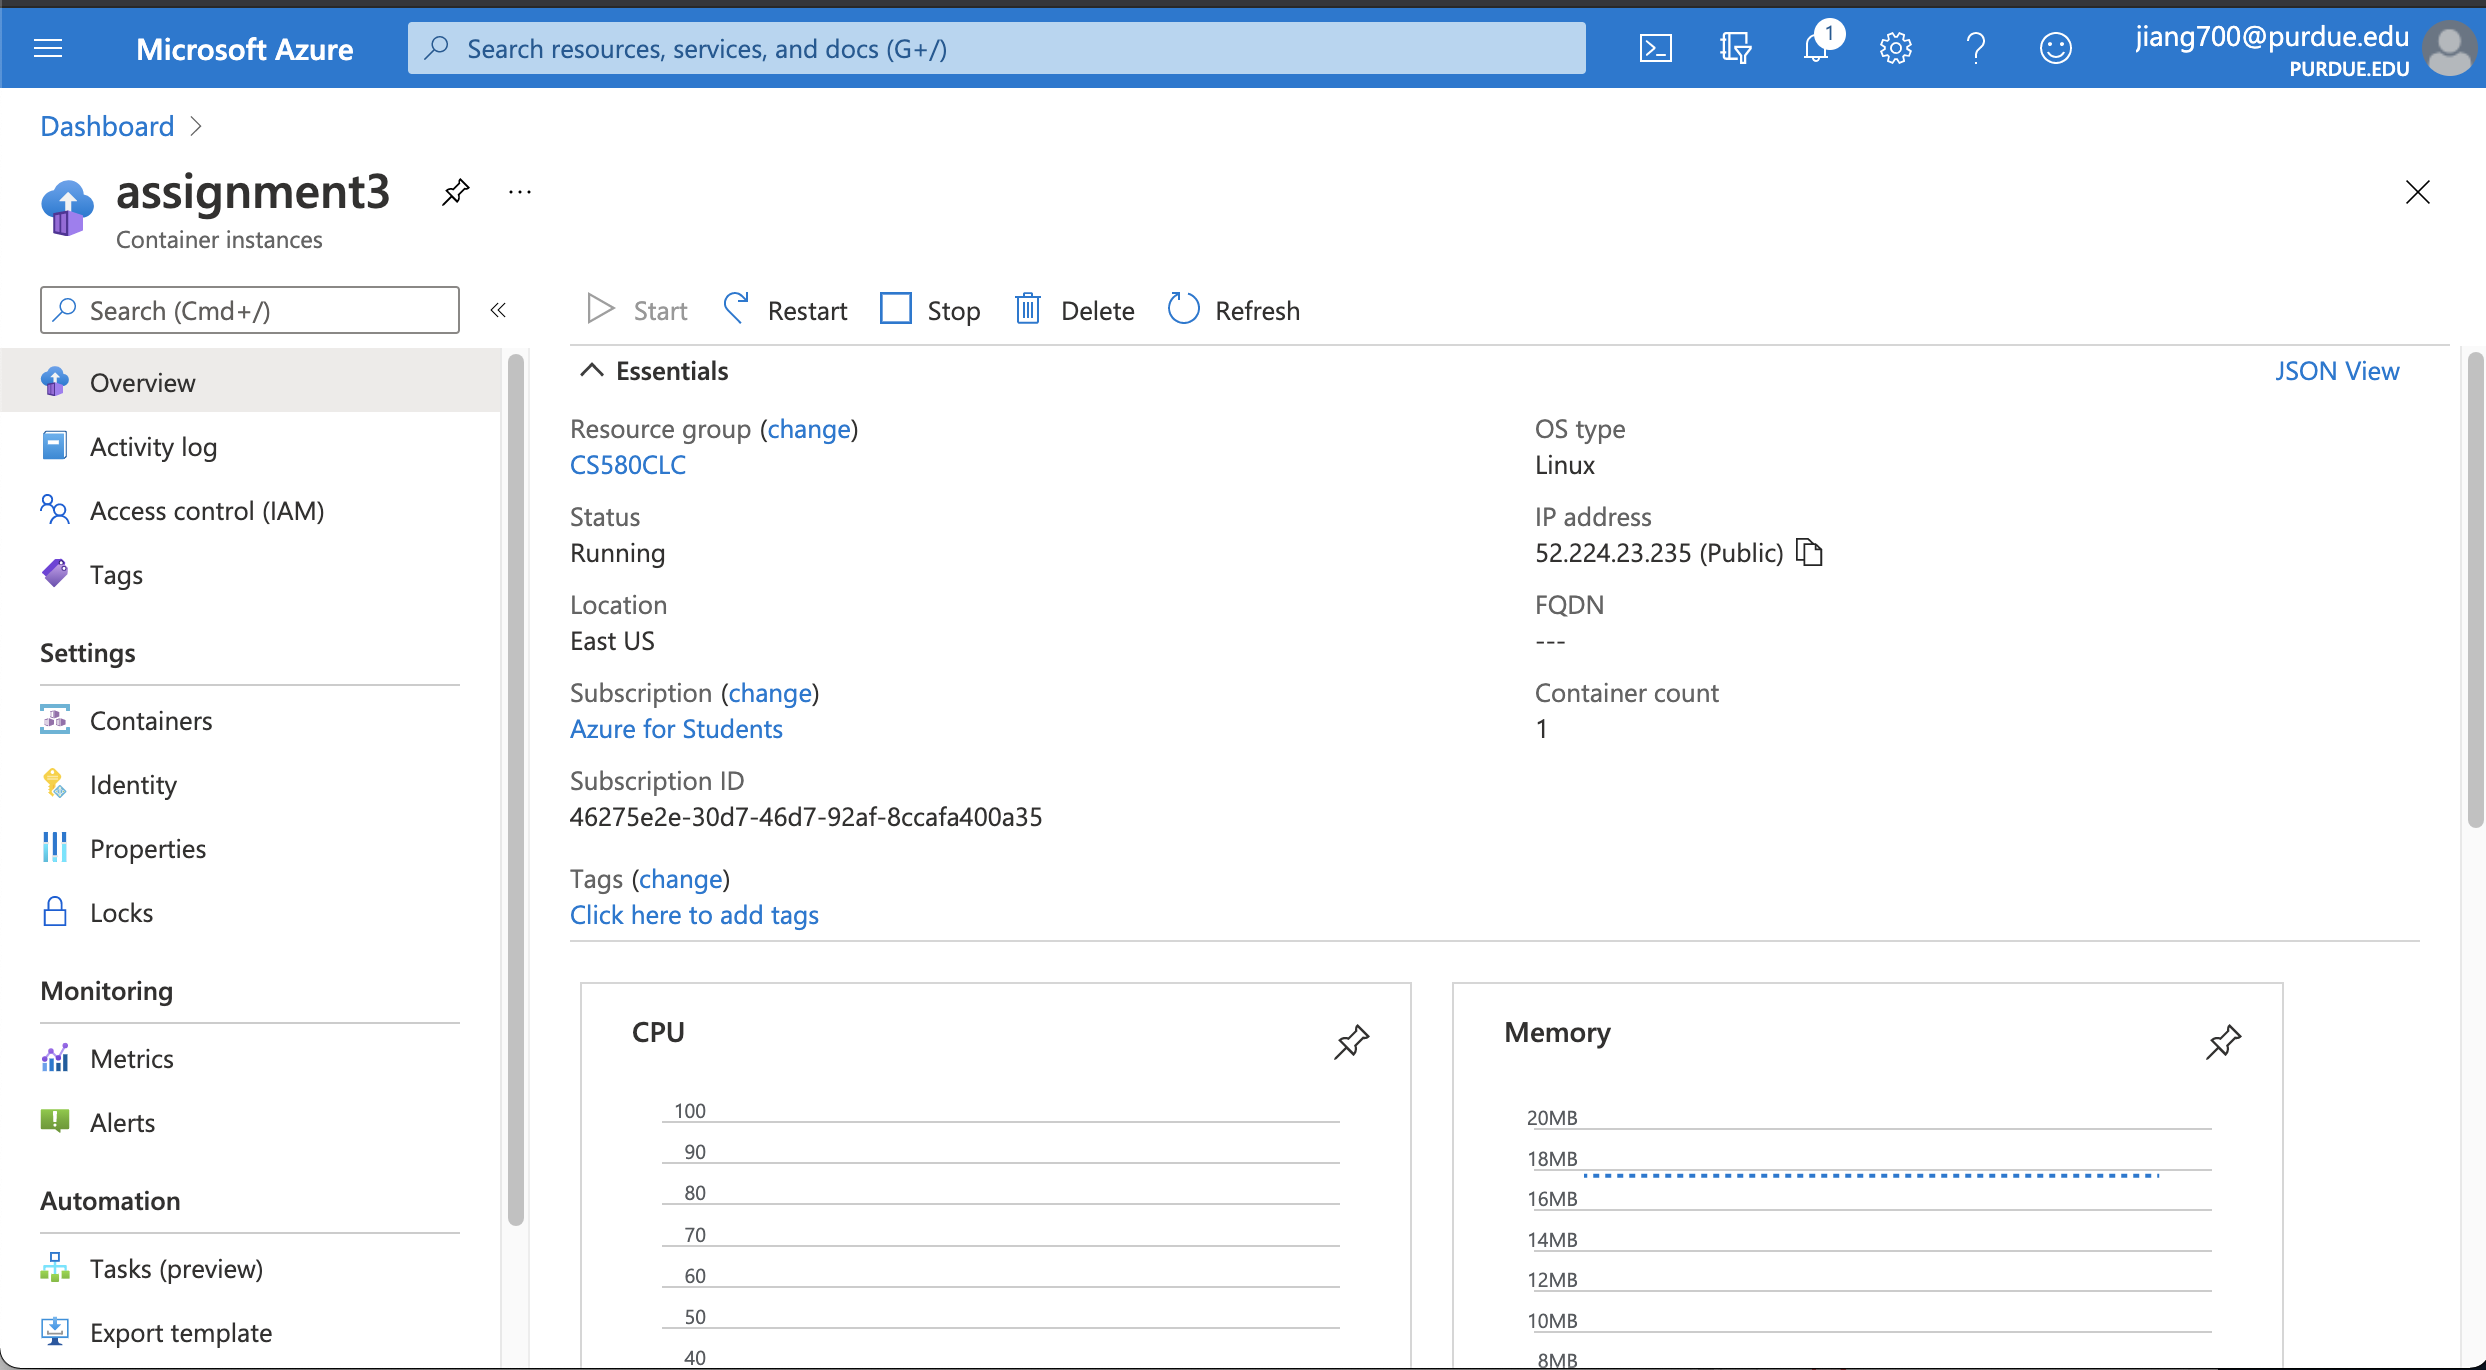
\includegraphics[scale=0.35]{ass3-2.png}

\section{Screenshot of container registry}
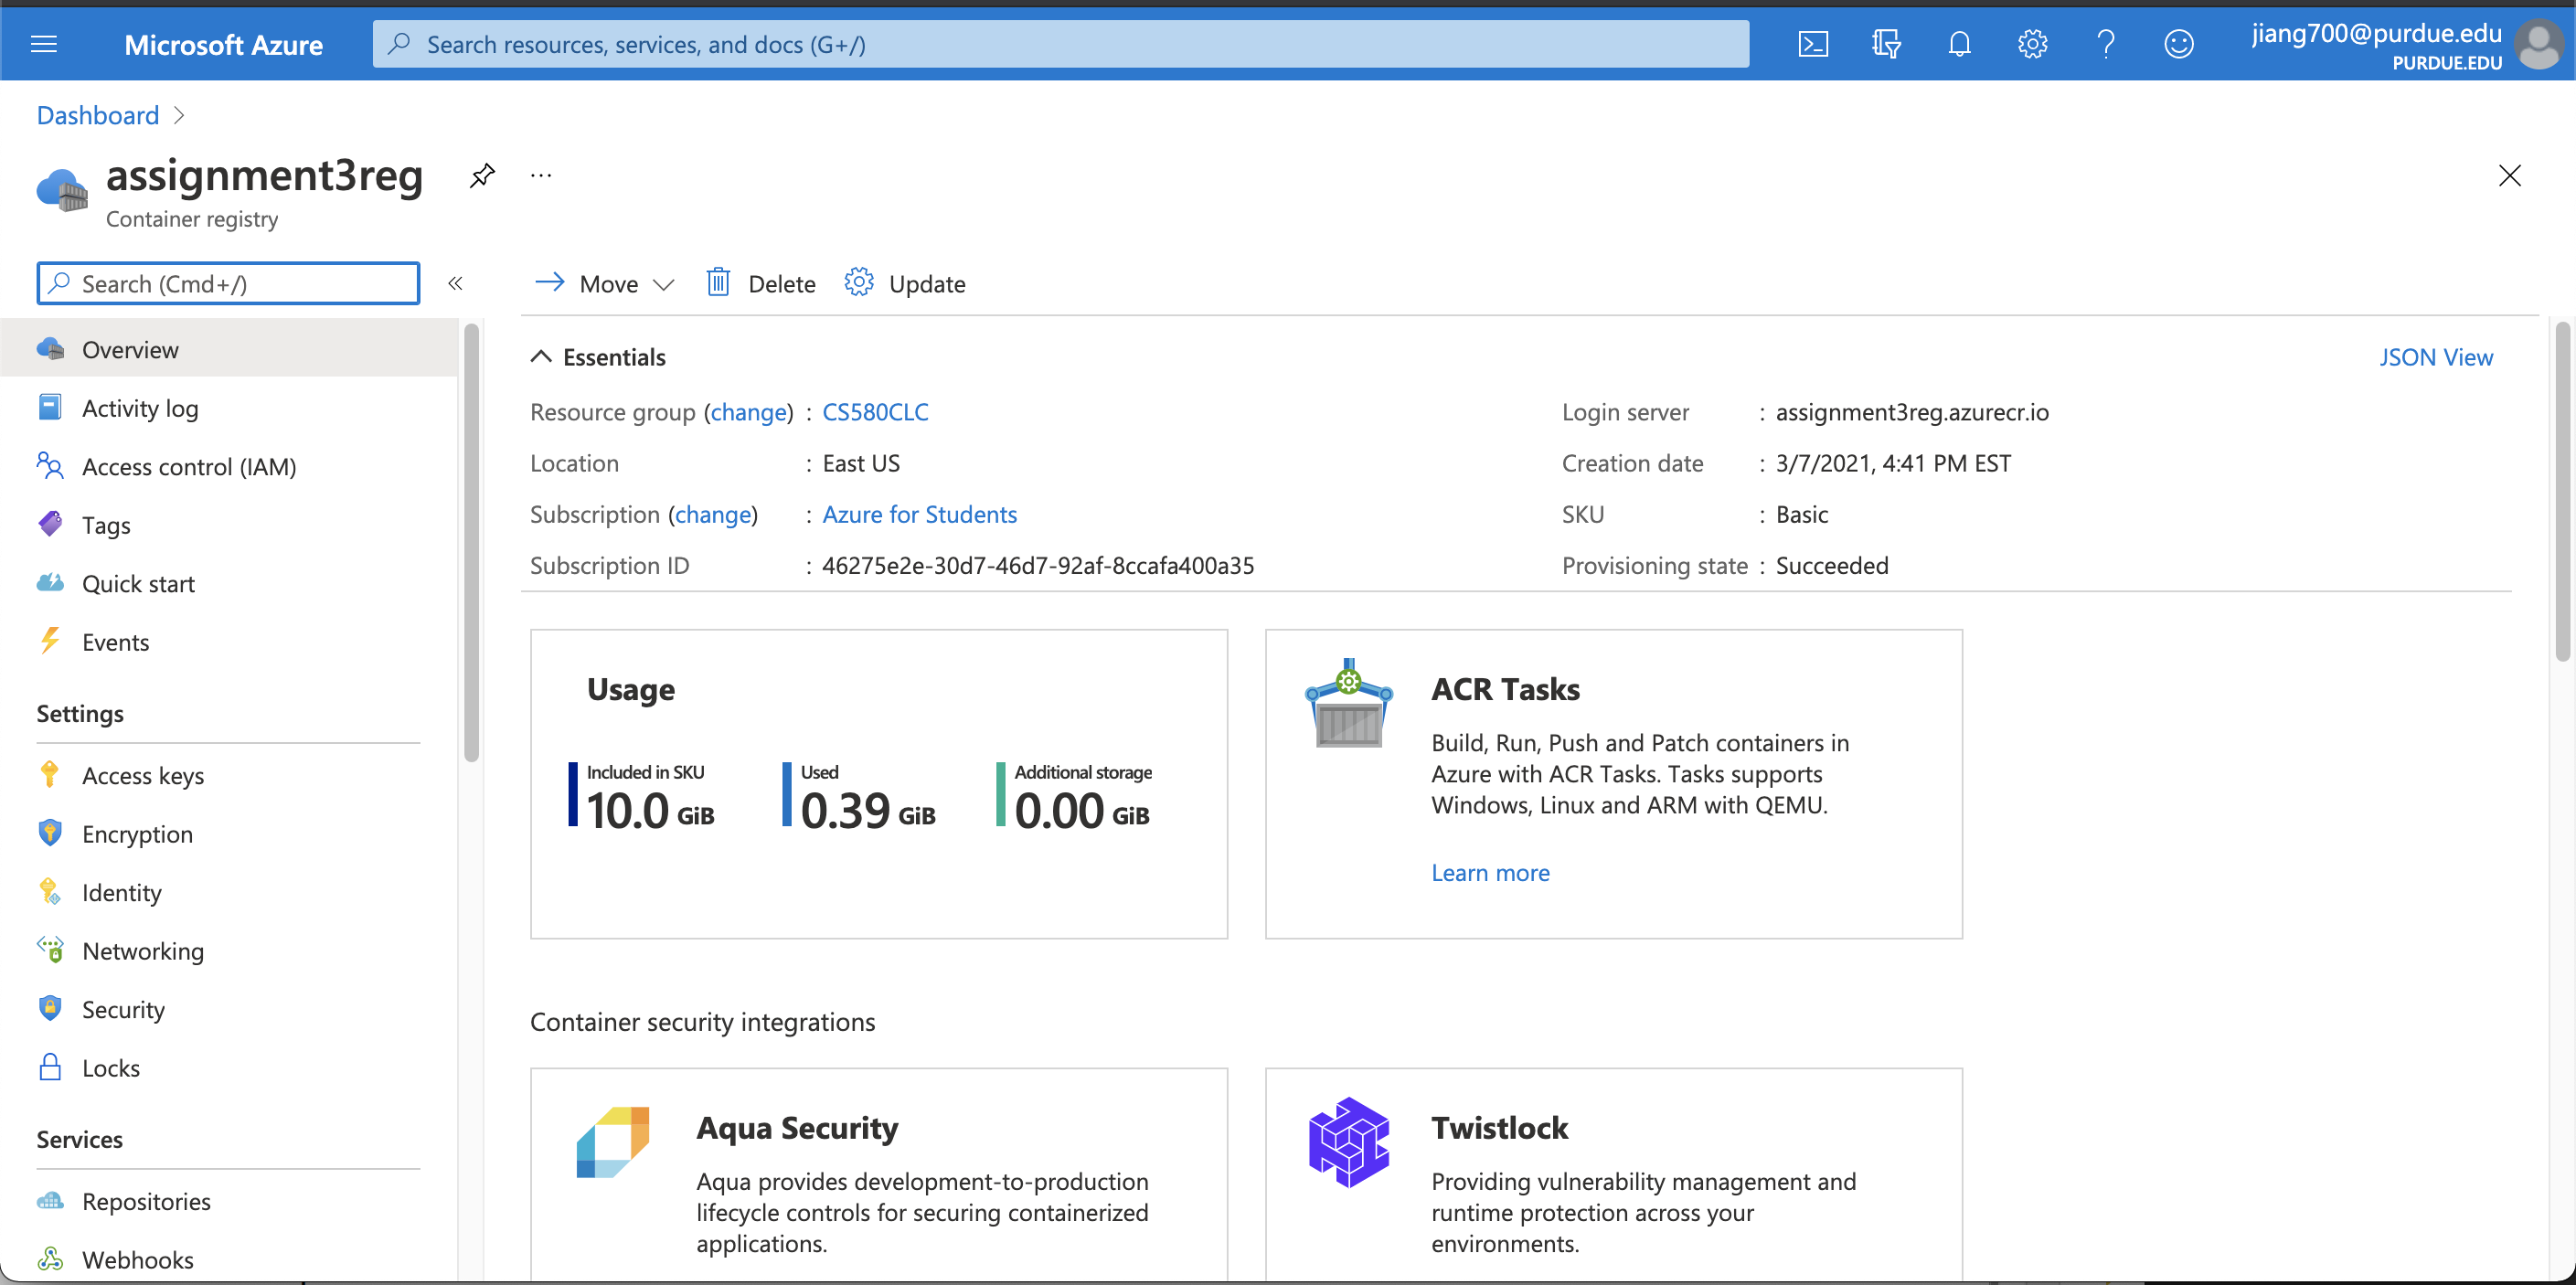
\includegraphics[scale=0.3]{ass3-3.png}

\section{Part 4}
In order to make the application work with Azure client, I first created a new instance of container running the RESTful application on Azure. Then, I modified my python script used in the previous assignment. Instead of using a hash code that represents local image, I passed the address of the running container I just created as input parameter to the program. After that, the python script can print out logs of the container running on Azure. 

\section{Analysis}
\begin{itemize}
    \item 1. The other options of SKU are standard and premium. Standard SKU has 100GB storage, 10 web hooks; premium SKU has 500GB storage and offers enhanced throughput for docker pulls across multiple, concurrent nodes. It also has 500 web hooks and supports Geo Replication.
    \item 2. If large user groups use admin user accounts, then too many users will have admin privileges, which will cause security issues.
    \item 3. It is very compatible. The Dockerfile doesn't need to be changed. We only need to change the dockerd command lines.
    \item 4. The procedure described in this assignment requires interaction with a graph UI and cannot be automated efficiently. Instead, I would write a script that performs the same setup and run it 1000 times.
\end{itemize}


\end{document}
